\chapter{Background}
\label{cha:background}

In order to understand how and why heterogeneous systems can be applied to the problem of
bitcoin mining, it is first important to obtain an understanding of how the bitcoin currency
works and what heterogeneous computing is.

\section{The Bitcoin Currency}
\label{sec:bitcoins}

Bitcoin, often abbreviated BTC, is a digital currency, using a peer-to-peer network to provide
a decentralized currency, not relying on banks or financial institutions to process transactions
or maintain accounts.

At the core of the bitcoin system is the block chain, a distributed, linked list consisting of blocks
which contains the transactions that have been executed on the network since the previous block was
generated.

A block is only valid if the arithmetic value of the double SHA-256 hash of its header is below
a certain target value. Finding a block that has such a header is computing intensive, and prevents
the network from being flooded with new blocks. The target value is decided by the network ``difficulty''
and is set to such a value that, on average, six new blocks are generated per hour.

To get people to participate in creating new blocks, a reward is offered to whomever manages to
create a block. This reward also ensures that more money is added into circulation. The size of
the reward decreases over time until a predetermined number of bitcoins have entered circulation.
The reward is currently 25 bitcoins and halves every 210~000 blocks. The total number of bitcoins
that is to be generated is 21~000~000 bitcoins. \cite{bitcoin}

\subsection{Mining Bitcoins}
\label{sec:bitcoin-mining}

The process of creating a new block for the bitcoin blockchain is often referred to as \textit{mining},
refering to the fact that a lot of energy may need to be expended in order to find a valid block.

The process begins with the creation of a transaction that transfers the reward for generating the block
into the account of the miner. This transaction is often called the coinbase or generation transaction.
All transactions transmitted to the bitcoin network since the last block was generated are gathered and
the hash of each transaction is inserted into a merkle tree.

The root of the merkle tree is inserted into the header for the new block together with the hash of the
previous block and various other fields specified by the standard. If the hash of the header is below the
target value, the block is successfully mined and transmitted to the network. If the hash does not satisfy
the demands of the network, a 32-bit field in the block header, called the \textit{nonce}, can be changed
to produce a new hash. In addition, transactions can be excluded in order to produce a different merkle
root for the header.

If more than one new block is pushed to the network at about the same time, the block chain diverges.
This situtation is resolved when the next block is generated; the longest block chain is then accepted
as the canonical block chain. \cite{bitcoin}

\subsection{Pooled Bitcoin Mining}

Because an increasing amount of computing power is being used to mine bitcoins, the difficulty of finding
a block has increased to such a level that no single bitcoin miner can hope to find a block on his or her
own. The current total hashing rate is about 396,5~EH/s\footnote{$396,5\cdot 10^{18}$} H/s) according to the
statistics available from \texttt{blockchain.info}. This means that the amount of work one can expect to
do in order to find a block is, on average, 237,9~ZH\footnote{$237,9\cdot 10^{21}$ hashes}! Using, for instance,
a GPU-based bitcoin miner with a hashrate of 1~GH/s, it would take, on average, $237,9\cdot 10^{14}$ seconds,
or 7~543~759 years to find a block.

To overcome this problem, mining pools were invented. A bitcoin mining pool is a service that distributes
work between miners. The work that is distributed has a lower target value than does the bitcoin network
itself, meaning that each participating miner can find valid blocks faster. Although most of the blocks
submitted to a pool does not fulfill the network requirements, sometimes a block does fulfill both the
pools difficulty requirements as well as the network requirements; in that case the new block is
submitted to the bitcoin network and all the miners who submitted work towards finding the block
is rewarded according to their contribution.

As such, pooled mining lets anyone with weaker hardware participate in bitcoin mining in exchange for
a smaller reward. However, using hardware such as regular CPUs and GPUs is still considered unprofitable
because of these processors' relative performance in comparison with specialized bitcoin mining ASICs.

\section{Existing Bitcoin Hardware}

Due to bitcoin's popularity and the possibility of profits, various specialized hardware has been used
to accelerate the process. Starting with simple programmes running on general-purpose processors,
bitcoin miners soon turned to GPUs in order to improve the performance and power efficiency of the
process. GPUs provide the possibility of running many hashing processes in parallel, in some cases
exceeding 1 GH/s\cite{bitcoin-hardware-cmp}. FPGA-based bitcoin mining hardware provide
better power efficiency than GPUs due to the possibility of tailoring the hardware design to
bitcoin mining.\todo{Move to related work?}

However, as bitcoin mining have become more profitable, ASIC-based bitcoin miners have taken over
the market and currently dominates in terms of performance and power efficiency, with performance
exceeding 200 GH/s \todo{reference http://www.spondoolies-tech.com/products/sp35-yukon-power-shipping-from-stock}
per chip\todo{Power?} \cite{bespoke-silicon}.

\section{Heterogenity and Dark Silicon}
\label{sec:dark-silicon}

Moore's law states that transistor density on integrated chips continue to double every
two years. In addition, native transistor speeds are increasing with a factor of 1,4.
According to Dennard scaling, which predicted that the power density of transistors, that
is the voltage and current used to operate the transistor, would scale down with the
size of the transistors, this would not be a problem; however, the energy efficiency
of transistors are only improving by a factor of 1.4, not keeping up with the scaling
of transistor size.

Under a constant power-budget, there is a shortfall of a factor of 2 in the energy budget,
and this utilization potential of a chip is falling exponentially by 2 times for each generation.
If the power limitation were to be based on the current generation, then designs would be 93,75\% dark in eight years.
This gives rise to the term ``dark silicon'', where a chip must either be underclocked or parts of
it turned off, giving rise to ``dark'' areas of the chip, in order to keep to a set power budget.
This is especially true for chips where the cooling solutions are no longer efficient enough to remove
the generated heat from a fully powered chip.

In order to work around this problem, the industry moved to using multicore processors around 2005.
However, adding multiple cores does not circumvent the problem in the long run.
Multicore chips will not scale as transistors shrink, and the fraction of a chip that can be filled with cores running at full frequency is dropping exponentially with each processor generation. 
Large fractions of the chip will be left dark - either switched off for a long time, or significantly underclocked.
Hence new designs are required, where new architectural techniques spend area to buy energy efficiency. \cite{dark-silicon}

\subsection{Approaches to the Problem of Dark Silicon}
To work around the problem of dark silicon, several approaches have been suggested as solutions.
There are four approaches areas suggested by Taylor\cite{dark-silicon}: Shrinking the chip, dimming the chip, specialization and so-called "Deus Ex Machina".
All four refer to a particular solution to the dark silicon issue.

%The need to work around the problem of dark silicon has lead to several approaches
%being suggested as solutions. In \cite{dark-silicon} Taylor describes a taxonomy called ``The four horsemen'',
%referring to the fact that none of the solutions appear to be ideal.
%These are four proposed responses that are emerging as solutions beyond making multicore chips \cite{dark-silicon2}.
%Taylor argues that future chips will apply not just one of these solutions, but all of them.
%It can be seen from the success of complex multi-regime devices like MOSFETs that engineering as a field has an enormous tolerance for complexity if the end result is better.

%The four horsemen are The Shrinking Horseman, The Dim Horseman, The Specialized Horseman and The Deus Ex Machina Horseman,
%each referring to a particular solution to the dark silicon issue. \cite{dark-silicon}

%\subsubsection{The Shrinking Horseman}
\subsubsection{Shrinking the chip}

Instead of having dark silicon on the chip, one may simply shrink the chip itself.
%Taylor\cite{dark-silicon} views these "shrinking chips" as the most pessimistic outcome.
Although all chips may eventually shrink somewhat, the ones that shrink the most will be those where dark silicon cannot be applied fruitfully to improve the product.
\todo{Nært overflødig?}These chips will rapidly turn into low-margin businesses for which further generations of Moore’s law provide small benefit.

Futhermore, there are other effects: Exponentially smaller chips are not exponentially cheaper, since mask cost, design cost and I/O pad aread cannot be amortized. 
Competition will most likely favor chips that utulizes dark silicon to improve overall product, causing chips that are only shrinked to sell at low market price, causing loss to the company.
And last, but not least, exponential shrinking leads to exponential rise in power density, and chip temperature will thus follow suit.
Meeting the temperature limit will reduce the scaling below the nominal 1,4x expected energy efficienty. \cite{dark-silicon}

%There are also second-order effects assosiated with shrinking chips:

%\begin{itemize}
%    \item Exponentially smaller chips are not exponentially cheaper.
%    In addition to the silicon itself, cost include mask costs, design costs and I/O pad area.
%    These cannot be amortized, and the price will increase per mm$^2$, as the chip shrinks.
%    \item Shrinking the silicon can also shrink the chip selling price, but competition will likely force companies to utilize dark silicon if it can attain a benefit for the end product.
%    Companies who would rely on shrinking only, may loose the competition and sell chips at catastrophically decreased chip prices.
%    \item Exponential shrinking leads to exponential rise in power density, and chip temperature will thus follow suit.
%    Meeting the temperature limit will reduce the scaling below the nominal 1,4x expected energy efficienty. 
%\end{itemize}

%\subsubsection{The Dim Horseman}
\subsubsection{Dimming the chip}
While the fractions of dark transistors of the chip increases exponentially, the silicon area become exponantially cheaper as resource, relative to power and energy consumption.
This gives the opportunity to spend area to buy energy efficiency, and basing new architectures on this.
\todo{Consider adding a figure to better illustrate the point}Dark silicon area can be populated with logic that is used only part of the time.
By employing heavy underclocking or infrequent use, large amount of otherwise-dark silicon area are put to productive use while meeting the power budget.
The term "dim silicon" refers to the techniques based on this approach.
The architecture has to strategically manage the chip-wide transistor duty cycle, to enforce the overall power constraint. 

\todo{Consider whether details of dim-silicon implementations/examples should be moved to related work.} The early 90-nm designs of, for instance, Cell and Prescott, were dimmed because actual power exceeded design-estimated power. 
Lately, more increasingly more elegant methods are converging, that make better trade-offs.
Among the dim silicon techniques are dynamically varying the frequency with the number of cores being used, scaling up the amount of cache logic, employing near threshold voltage (NTV) processor designs, and redesigning the architecture to accommodate bursts that temporarily allow the power budget to be exceeded, such as Turbo Boost and computational sprinting. \cite{dark-silicon}

% %\todo{This subchapter ended up long. Try to see if it can be reduced. Especially NTV}
%According to Taylor\cite{dark-silicon}, as exponentially larger fractions of a chip’s transistors become dark transistors, silicon area becomes an exponentially cheaper resource relative to power and energy consumption.
%Therefore new architectural techniques that spend area to buy energy efficiency is called for.
%Instead of shrinking silicon, one may consider populating dark silicon area with logic that is used only part of the time, and interesting new design possibilities occurs.
%The term "dim silicon" refers to techniques that put large amounts of otherwise-dark silicon area to productive use by employing heavy underclocking or infrequent use to meet the power budget.
%The architecture has to strategically managing the chip-wide transistor duty cycle to enforce the overall power constraint. 
%Whereas early 90-nm designs such as Cell and Prescott were dimmed because actual power exceeded design-estimated power, more increasingly more elegant methods are converging, that make better trade-offs.
%Among the dim silicon techniques are dynamically varying the frequency with the number of cores being used, scaling up the amount of cache logic, employing near threshold voltage (NTV) processor designs, and redesigning the architecture to accommodate bursts that temporarily allow the power budget to be exceeded, such as Turbo Boost and computational sprinting.

% %\todo{Consider shorting down or removing entire lists from each sub-chapter, to keep the four horsemen short and concise.}Amond dim silicon methods are: 

%\begin{itemize}
%    \item Turbo boost, where less core are active, the higher the frequency they may run at.
%    Energy gained from turning off cores is used to increase voltage and frequency of active cores.
%    This is known as Dynamic voltage and frequency scaling (DVFS).
%    \item Near-threshold voltage (NTV) Processors.
%    Transistors were at 2013 operated around 2,5x the threshold voltage, an energy-delay optimal point. 
%    This is at a point where reducing the voltage severely affects the frequency drop, which reduces the effective gain from downward-DVS.
%    Nevertheless, researchers have begun exploring this regime.
%    NTV logiv is a recent approach, where transistors in the near-threshold regime are operated slightly above the threshold voltage.
%    This provides a more palatable trade-off between energy and delay than subthreshold circuits, for which frequency drops exponentially with voltage decreases.
%    \todo{Give a proper mention of where the following numbers were taken from}
%    Although NTV per-processor performance drops faster than the corresponding savings in energy-per-instruction (5X energy improvement for an 8x performance cost), the perfor- mance loss can be offset by using 8x more processors in parallel if the workload allows it.
%    Then, an additional 5x processors could turn the energy efficiency gains into additional performance. 
%    \todo{Have to admit, I still don't understand how this is a gain. And this is almost the point of too much. Should remove the example, and find a different way to explain}So, with ideal parallelization, NTV could offer 5x the throughput improvement by absorbing 40x the area. 
%    But this would also require 40x more free parallelism in the workload relative to the parallelism consumed by an equivalent energylimited super-threshold many-core processor.
%    \item Bigger caches.
%    Because only a subset of cache transistors (such as a wordline) is accessed each cycle, cache memories have low duty cycles and thus are inherently dark. 
%    Adding cache is therefore one way to simultaneously increase performance and lower power density per square millimeter.
%    But the less memory-bound a running application is, the less the benefit.
%    \item Computational sprinting and turbo boost.
%    One temporarily exceeds the nominal thermal budget but relies on thermal capacitance to buffer against temperature increases, and then ramp back to a comparatively dark state.
%    These are used within "race to finish" computations.

%\end{itemize}

%\subsubsection{The Specialized Horseman}
\subsubsection{Specialization}
Specialization means that each within a set of processors, each are specialized for a subset of tasks, increasing energy efficiency or speed than a general purpose processor, for those particular tasks.
Any application are executed on the processor which is deemed as the most efficient.
Cores not in use are power- and clock gated, and thus do not waste energy unnecessarily.

Specialized accelerators already exist today that span diverse areas, including baseband processing, graphics, computer vision and media coding.
These enable orders-of-magnitude improvements in energy efficiency and performance, especially for computations that are highly parallel.
Systems with more coprocessors than general purpose processors is anticipated to rise, referred to as coprocessor-dominated architectures, or CoDAs.

Challenges with these systems are expected as well, one of them beeing the so-called "Tower of Babel" crisis.
\todo{Couldn't find a better way to state this without making it look like the source material. Have a look at it before deadline}The notion of general-purpose computation is fragmented, and the former clear lines of communication between programmers and software and the underlying hardware is eliminated.
For instance, CUDA for NVidia GPUs cannot be used for similar architectures, such as AMD.
There are several cases of overspecialization problems between accelerators, so that they cannot be used for closely related classes of computaion.
\todo{A little similar to source, see if this can be further written with own words}Then there are also adoption problams that is due to excessive cost of programming heterogeneous hardware (for instance, Sone Playstation 3 vs. Microsoft XBox), and specialized hardware risk becomming obsolete when standards are revised. \cite{dark-silicon}.









%This is the use of dark silicon to implement a host of specialized processors.
%They can be more energy efficient, or much faster than a general purpose processor.
%Programs are executed where it is most efficient.
%Unused cores are power- and clock gated in order to keep them from wasting energy.

%Specialization is already being realized today in forms of specialized accelerators that span diverse areas such as baseband processing, graphics, computer vision, and media coding.
%These accelerators enable orders-of-magnitude improvements in energy efficiency and performance, especially for computations that are highly parallel.
%It is expected to see a rise of systems with more coprocessors than general processors.
%Tayler refers to them as coprocessor- dominated architectures, or CoDAs.

%One of the expected challenges it the so-called "Tower of Babel" crisis, as the notion of general-purpose computation is fragmented, and the traditional clear lines of communication between programmers and software and the underlying hardware is eliminated.
%For instance, CUDA for NVidia GPUs is not usable for similar architectures, such as AMD.
%Overspecialization problems between accelerators that cause them to become inapplicable to closely related classes of computation has been observed.
%In addition, adoption problems are also caused by the excessive costs of programming heterogeneous hardware (such as Sony Playstation 3 vs. Microsoft XBox), and there is always the risk that specialized hardware may become obsolete as standards are revised. \cite{dark-silicon}.

%\todo{The following sections are expanding challenges to the specialized horseman, beyond the basic. Consider carefully if this delves in too deply of our own project report, and delete it all if so.}
%The following challenges needs to be adressed:
%\begin{itemize}
%    \item To combat the "Tower of Babel" problem, it is required to define a new paradigm for how specialization is expressed and exploited in future processing systems. 
%    New scalable architectural schemas that employ pervasively specialized hardware to minimize energy and maximize performance are needed. At the same time they need to insulate the hardware designer and programmer from such systems’ underlying complexity.
%    \item  Amdahl’s law adds issues for specialization.
%    To save energy across the majority of the computation, broad-based specialization approaches that apply to both regular, parallel code and irregular code must be found.
%    It must also be ensured that communicating specialized processors doesn’t fritter away their energy savings on costly cross-chip communication or shared-memory accesses. 
%    \item Recent efforts. The UCSD GreenDroid processor. \todo{YEP!}Proposal: This is an example. Move and describe it in related works.
%\end{itemize}

%\subsubsection{The Dues Ex Machina Horseman}
\subsubsection{Dues Ex Machina}
The termology "Deus ex machina" from literature or theater, in which the protagonists seem increasingly doomed until the very last moment, when something completely unexpected comes out of nowhere to save the day.
In the case for dark silicon, one deus ex machina would be a breakthrough in semiconductor devices.
The required breakthrough would have to be very fundamental, making it possible to build transistors out of devices other than MOSFETs. 
There are physical limits to what can be done with \todo{I chose to not elaborate this one further}leakage from MOFSET transistors, and transistors made of other devices can go beyond these limits.
New transistors must also be able to compete with MOFSETs in performance.
Tunnel field-effect transistors (TFET) and nanoelectromechanical system (NEMS) switches are examples on inventions that hint to order-in-magnitude improvements in the leakage problem, but they still fall short in performance.
Overall, this is the most unpredictable field of solution. \cite{dark-silicon}



%Taylor notes that this one is the most unpredictable\cite{dark-silicon}.
%He uses the termology "Deus ex machina" from literature or theater, in which the protagonists seem increasingly doomed until the very last moment, when something completely unexpected comes out of nowhere to save the day.
%In the case for dark silicon, one deus ex machina would be a breakthrough in semiconductor devices.
%The required breakthrough would have to be very fundamental, making it possible to build transistors out of devices other than MOSFETs. 
%There are physical limits to what can be done with \todo{I chose to not elaborate this one further}leakage from MOFSET transistors, and transistors made of other devices can combat this.
%New transistors must also be able to compete with MOFSETs in performance.
%Tunnel field-effect transistors (TFET) and nanoelectromechanical system (NEMS) switches are examples on inventions that hint to order-in-magnitude improvements in the leakage problem, but they still fall short in performance.

% Please rewrite the above, the word "horseman" is something we shouldn't use.

\section{Heterogeneous Architectures}
\label{sec:heterogeneous}
\todo{Used as head chapter, but consider removal if SHMAC is the only heterogeneous computer described.}Heterogeneous multiprocessor contains of specialized processors for different classes of applications, and are the implementation of the specialization approach.
One such system is the Single-ISA Heterogeneous MAny-core Computer (SMHAC), which is a research project 
initiated by EECS on NTNU. \cite{shmac-plan}

\subsection{The Single-ISA Heterogeneous MAny-core Computer}
\label{sec:shmac}
The Single-ISA Heterogeneous MAny-core Computer is an architecture for investigating heterogeneous systems at all abstraction levels, as illustrated in figure \ref{fig:shmacAbstractionLevels}.
%The point is to create a flexible framework in which different heterogeneous processors can be created from a collection of processing elements and accelerators. % - Not anymore?
The programming model is kept constant across SHMAC-instances, while the underlying implementation changes.
This way, software design space exploration is facilitated.
It implements a tile-based architecture with a mesh interconnect. All processor tiles implement the same
ARM ISA and the same memory model, in order to achieve a common programming model \cite{shmac-plan}.
An illustration of SHMAC can be seen in figure \ref{fig:shmac}.

\begin{figure}[htb]
    \centering
    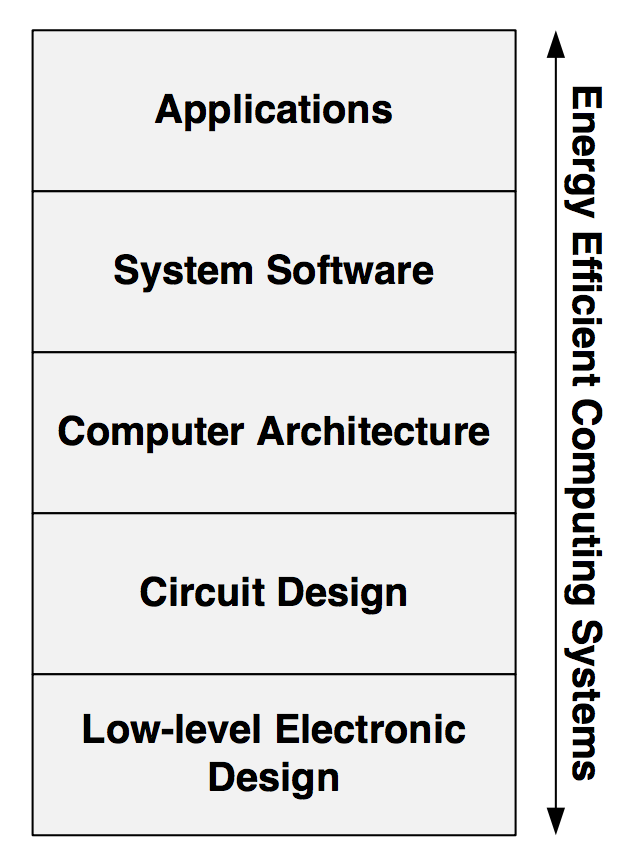
\includegraphics[width=0.5\textwidth]{Figures/Heterogeneous/SHMACAbstractionLevels}
    \caption{Levels of abstraction in computing systems \cite{shmac-plan}.}
    \label{fig:shmacAbstractionLevels}
\end{figure}

\begin{figure}[htb]
    \centering
    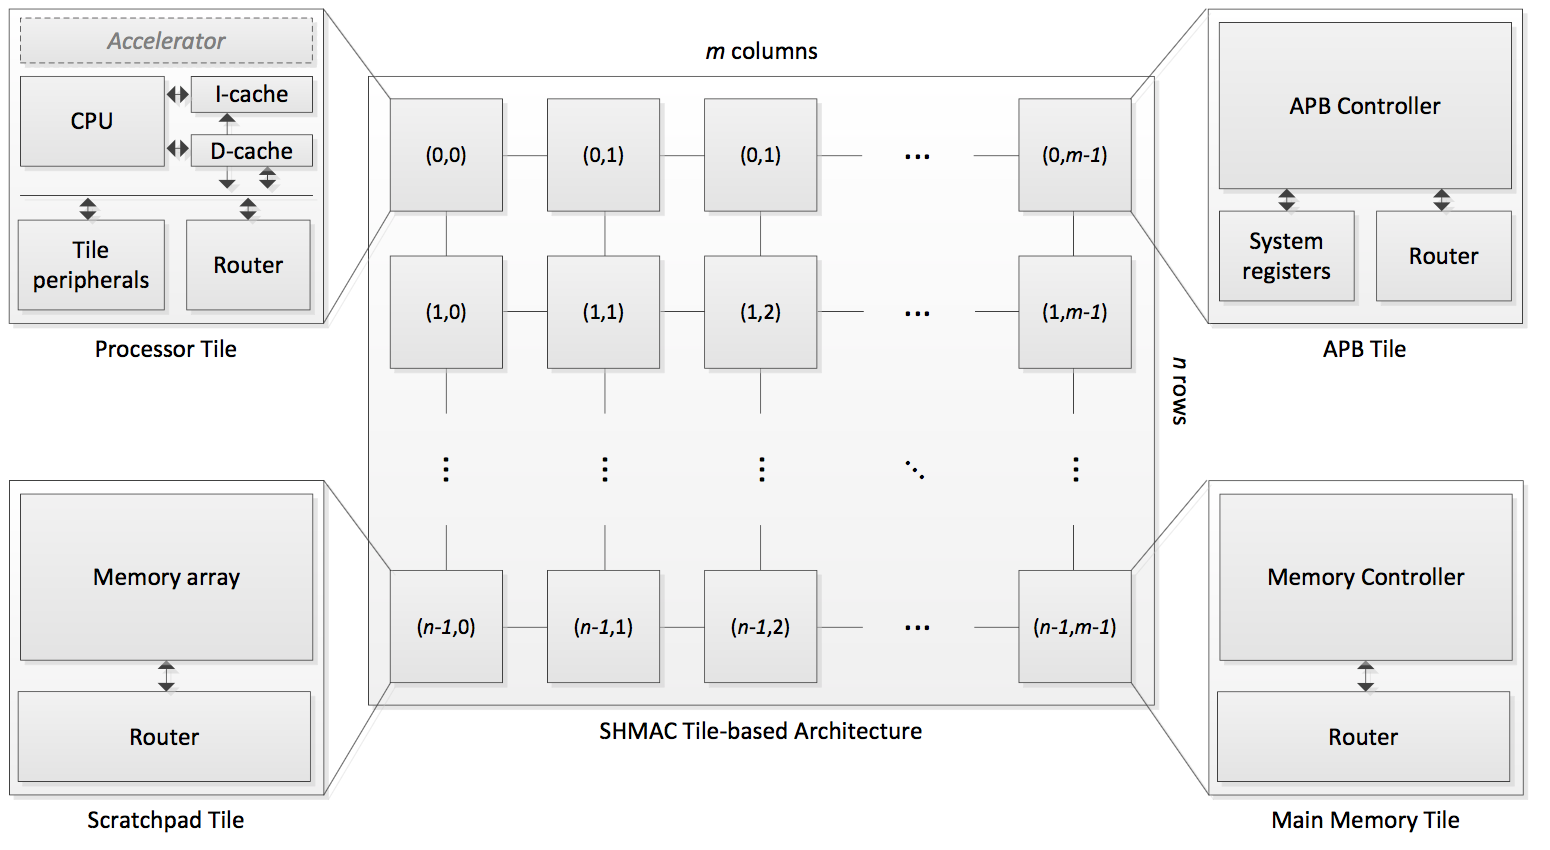
\includegraphics[width=0.95\textwidth]{Figures/Heterogeneous/SHMAC}
    \caption{High-Level architecture of SHMAC \cite{shmac-plan}.}
    \label{fig:shmac}
\end{figure}

%\todo{PROBLEM: This paragraph is way too similar to original text. Must fix, one way or another. }NTNU argues that the SHMAC-approach gives the right tools to reach the research goles outlined in the plan in \cite{shmac-plan}.
%For software research, SHMAC makes it possible to explore substantially more diverse systems than the ones currently provided by the industry.
%Furthermore, SHMAC-based computers realized in FPGAs will be significatly faster than using simulators.
%It is expected that co-developing software and hardware will result in new knowledge that gives insight into both hardware and software issues.
%Micro- and macro-architecture components can also be combined with novel transistor technologies and ASIC realizations to reach research goals at even lower abstraction levels.

% - Yes, I commented out this stuff: write what you want to say, then use citations to back it up - do not copy from the citations!

%We believe that the SHMAC-approach gives us the right tools to reach the research goals outlined in this plan. For software research, SHMAC makes it possible to explore substantially more diverse systems than those cur- rently provided by the industry. At the same time, SHMAC-architectures realized in FPGAs will be significantly faster than simulator-based approaches. We expect that co-developing software and hardware result in substan- tial cross-fertilization that gives insights into both hardware and software issues. Finally, the SHMAC micro- and macro-architecture components can be combined with novel transistor technologies and ASIC realizations to reach research goals at the lower abstraction levels.

\subsubsection{SHMAC Architecture}

SHMAC is a tile-based architecture, with the processing elements laid out in a rectangular grid with neighbour-to-neighbour connection, using a mesh interconnect, using XY-routing.
%Several tile types are currently supported, not including the tile described in this report,
%with the most important ones being the processor tile, which contains a Turbo Amber CPU
%\footnote{See section \ref{sec:aht} for a short overview}, a scratchpad tile which functions as
%fast temporary storage, a DRAM tile and an I/O tile for communicating with a host system.

The supported tile types, not including the tile described in this report, are the following:
\todo{Entire following list pretty much rip-off, except Amber and Turbo Amber. Sources from elsewhere needed.}
\begin{description}
  \item[Amber Processor Tile] Processor tile that contains an ARM Amber processor, caches, peripherals and optional accelerators.
  It can be seen in figure \ref{fig:shmac-cpu}.
  \todo{This and next 2 sentences rip-off.}Currently, the peripherals consists of interrupt controller, timers and tile registers.
  The tile registers are per-tile memory that store local information like the processor ID, the coordinates of the tile, etc. 
  The caches, router and peripherals are connected to a Wishbone bus.
  
%  \todo{IMPORTANT! Affected our results!}Caches reduce the average memory latency, but adding caches also add the possibility for coherence problems.
%  This is currently solved by placing shared data in uncachable memory regions, through software. 
%  
  The processor tile can be equipped with optional accelerators, designed to execute a specified computation in a very effective way.
%  
%  
  \item[Turbo Amber Processor Tile] \todo{Suggest source needed from Redmine or the internet}Same as previous, but has an ARM Turbo Amber processor with \todo{Needs to be confirmed} higher performance.
  \item[Scratchpad Tile] Includes memory and a router, but no processing element. 
  It is is an on-chip memory where the contents are managed by software (e.g. programmer, compiler, system software, etc.).
  Each scratchpad tile is given a 128 MB address space.
  The number of scratchpad tiles depends on a number of factors like the amount of block RAM available on the chosen FPGA, the desired access latency, the amount of block RAM used for caches in the processor tiles and the possibility of access contention\cite{shmac-plan}.
  The memory layout for SHMAC is seen in figure \ref{fig:shmac_memory}.
  \item[Main Memory Tile] Memory controller tile that gives SHMAC access to off-chip memory.
  \item[APB Interface] This tile implements the Advanced Peripherals Bus (APB) slave which gives the host processor on the Versatile boards access to SHMACs memory space. 
  In addition, the APB contains system registers which are used for managing communication with the host system.
  \item[Dummy Tile] Contains only a router and is used to fill remaining tiles when there is not enough resources available in the target FPGA to fill all tiles with tiles that implement functionality.\end{description}


\begin{figure}[htb]
    \centering
    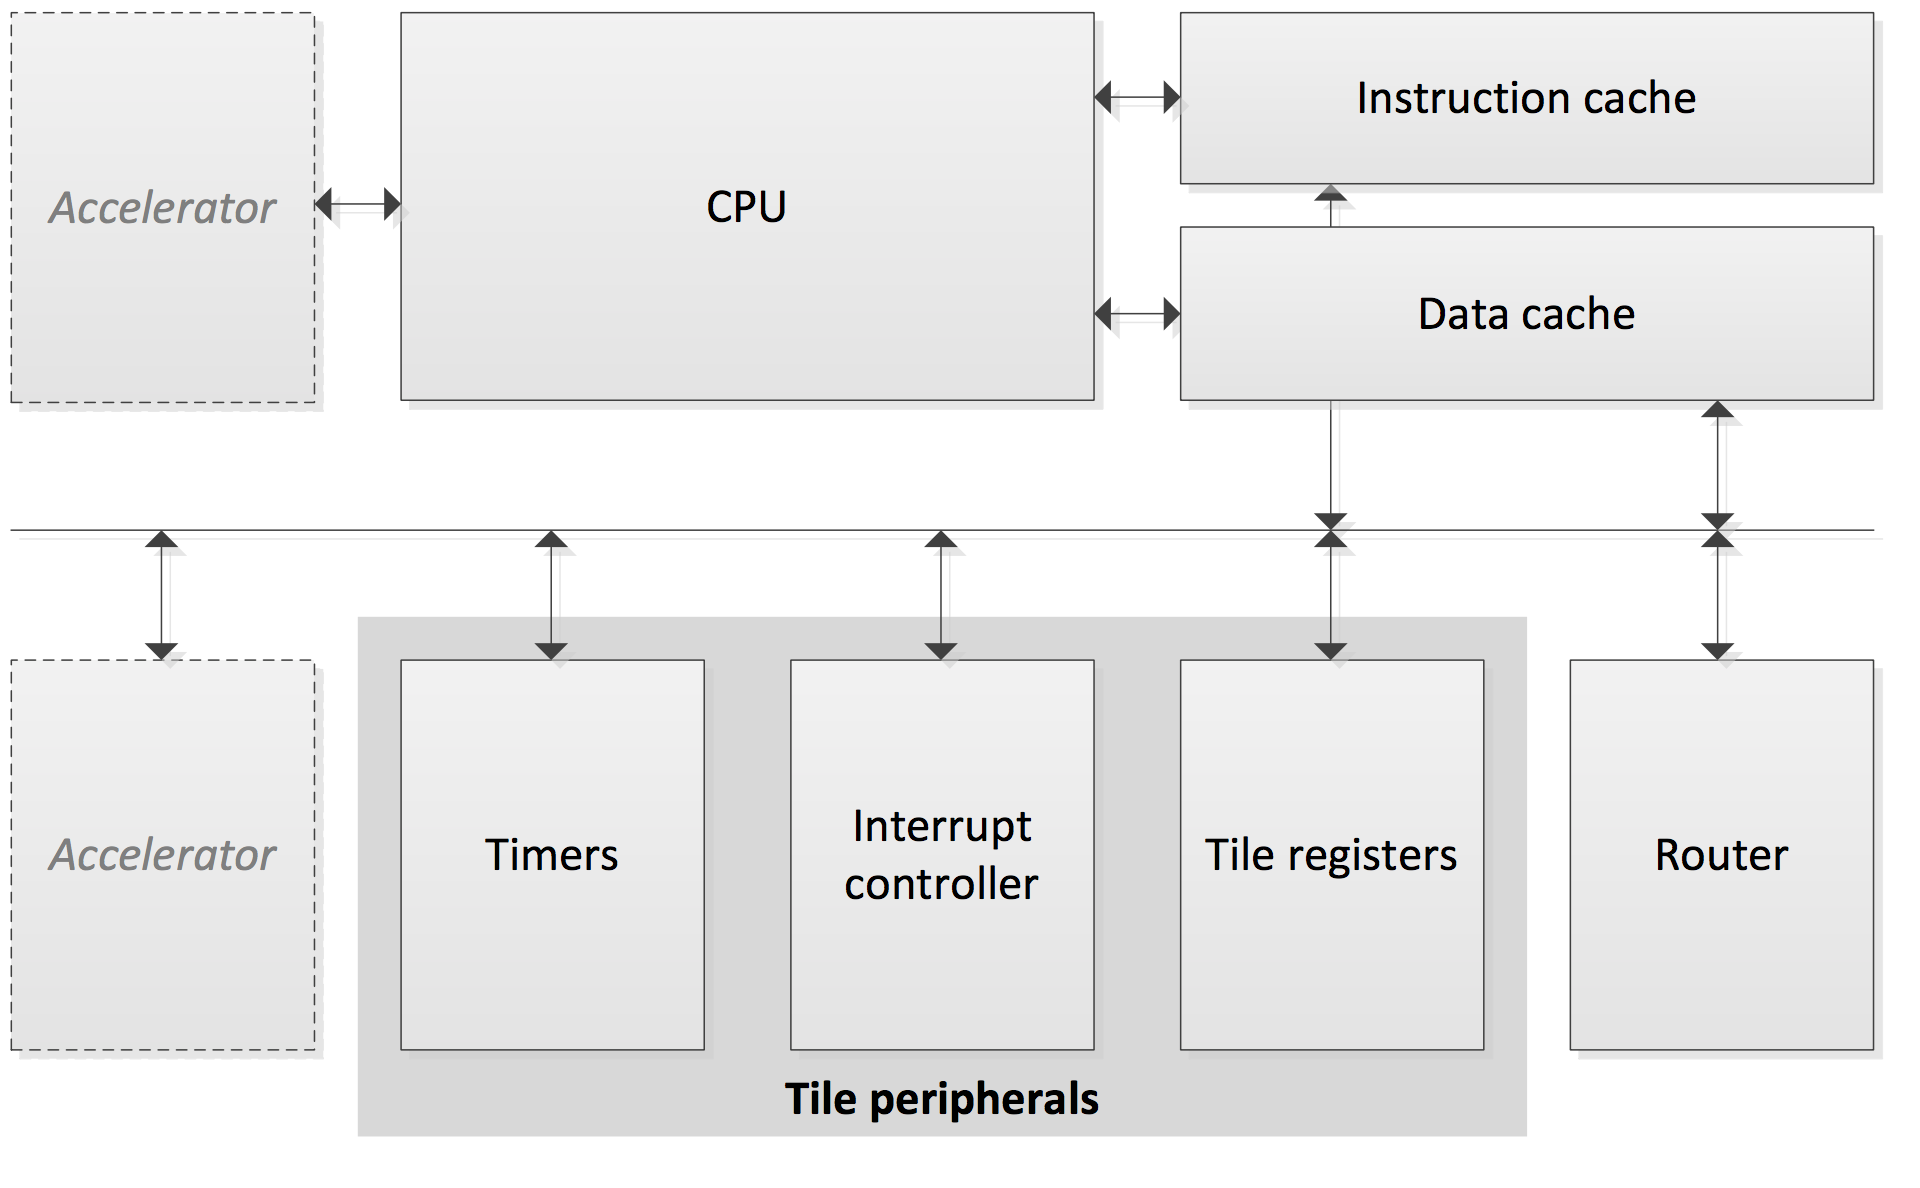
\includegraphics[width=1.0\textwidth]{Figures/Heterogeneous/SHMACCPU}
    \caption{SHMAC Processor tile \cite{shmac-plan}.}
    \label{fig:shmac-cpu}
\end{figure}


\subsubsection{SHMAC Memory Map}

Figure \ref{fig:shmac-memory} shows how the memory is mapped in ARM-based SHMAC.

The Exception table contains 8 instructions, one for each exception type described on \todo{Not mentioned so far in this document. Consider inclusion}Redmine.
\todo{Rip-off}The high end of the memory space is reserved for system registers and tile registers. 
The tile registers are private for each tile and contain information like the tiles coordinates and other useful data while the system registers are used for communication with the host system.

%The scratchpad tiles have been given a 128 MB address space. The SHMAC architecture supports 1 to k scratchpad tiles where k can be chosen independently of the number of tiles in the SHMAC instance. The number of scratchpad tiles depends on a number of factors like the amount of block RAM available on the chosen FPGA, the desired access latency, the amount of block RAM used for caches in the processor tiles and the possibility of access contention.

\begin{figure}[htb]
    \centering
    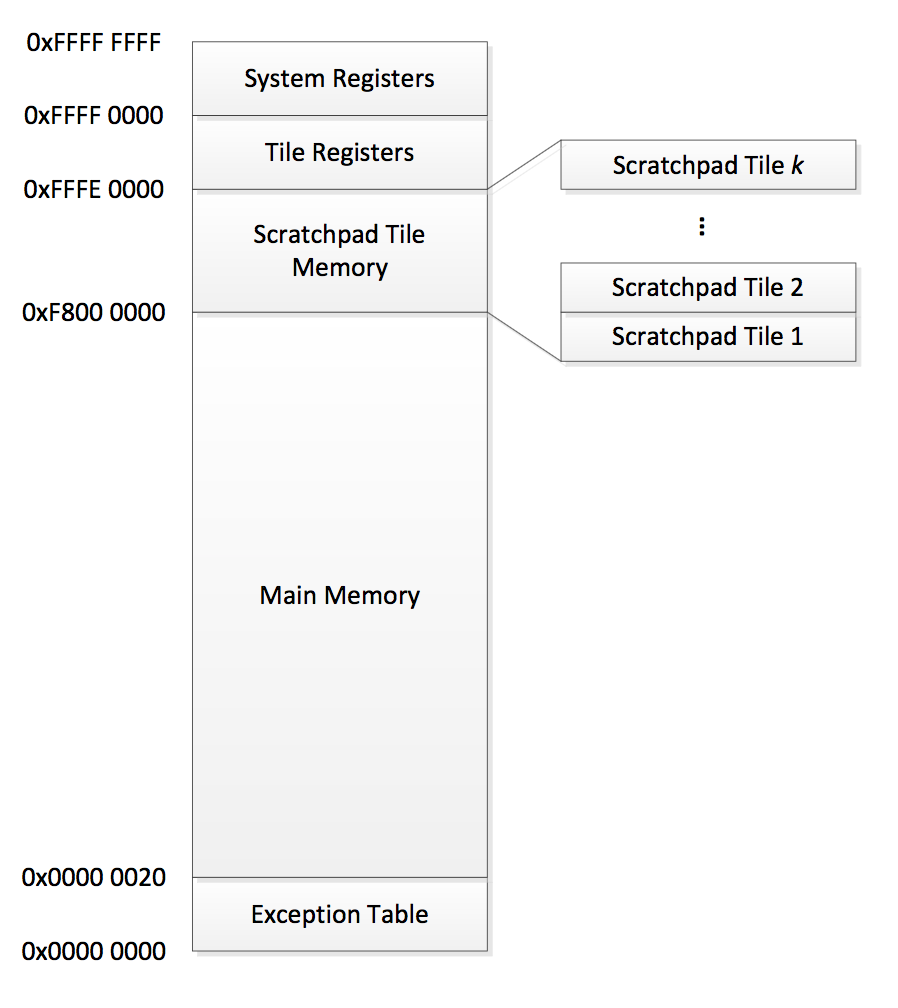
\includegraphics[width=1.0\textwidth]{Figures/Heterogeneous/SHMACMemory}
    \caption{Memory map of ARM-based SHMAC, as seen in \cite{shmac-plan}.}
    \label{fig:shmac-memory}
\end{figure}


%\subsubsection{Work packages}


